\section{Dữ liệu và thiết kế thí nghiệm}
\label{sec:data_experimental_design}

\subsection{Tập dữ liệu Thực nghiệm và Phân tích Khám phá (EDA)}
Thí nghiệm được tiến hành trên tập dữ liệu chính thức của cuộc thi \textit{IISE PG\&E Energy Analytics Challenge 2025}, được lưu trữ mở trên nền tảng Zenodo với mã định danh số DOI \url{10.5281/zenodo.17085273}~\cite{pge2025zenodo}.
\begin{itemize}
    \item \textbf{Phạm vi không gian và thời gian:} Dữ liệu bao gồm chuỗi thời gian liên tục theo từng giờ kéo dài 3 năm liên tiếp (từ ngày 01/01/2020 đến hết ngày 31/12/2022) thuộc địa bàn phục vụ của PG\&E tại California.
    \item \textbf{Kích thước mẫu:} Tổng cộng 26,304 điểm quan sát theo giờ. Trong đó, tập huấn luyện công khai gồm 2 năm đầu tiên (Year 1: 2020 có 8,784 giờ do là năm nhuận; Year 2: 2021 có 8,760 giờ; tổng cộng 17,544 giờ). Tập kiểm tra độc lập (Year 3: 2022) bao gồm 8,760 giờ. Dữ liệu chất lượng cao, không có giá trị khuyết thiếu.
    \item \textbf{Biến mục tiêu phụ tải (\textit{Target Load}):} Công suất điện tiêu thụ đo bằng Megawatt (MW), dao động từ xấp xỉ 1,500~MW (ban đêm mùa xuân) lên tới hơn 4,200~MW (buổi chiều nắng nóng đỉnh điểm tháng 7 và 8).
    \item \textbf{Biến ngoại sinh khí tượng:} Ghi nhận nhiệt độ bề mặt ($^\circ\text{C}$) và bức xạ mặt trời trực tiếp GHI ($\text{W/m}^2$) từ 5 trạm quan trắc địa lý phân tán (Site-1 đến Site-5).
\end{itemize}

\begin{figure}[htbp]
    \centering
    \begin{subfigure}[b]{0.48\textwidth}
        \centering
        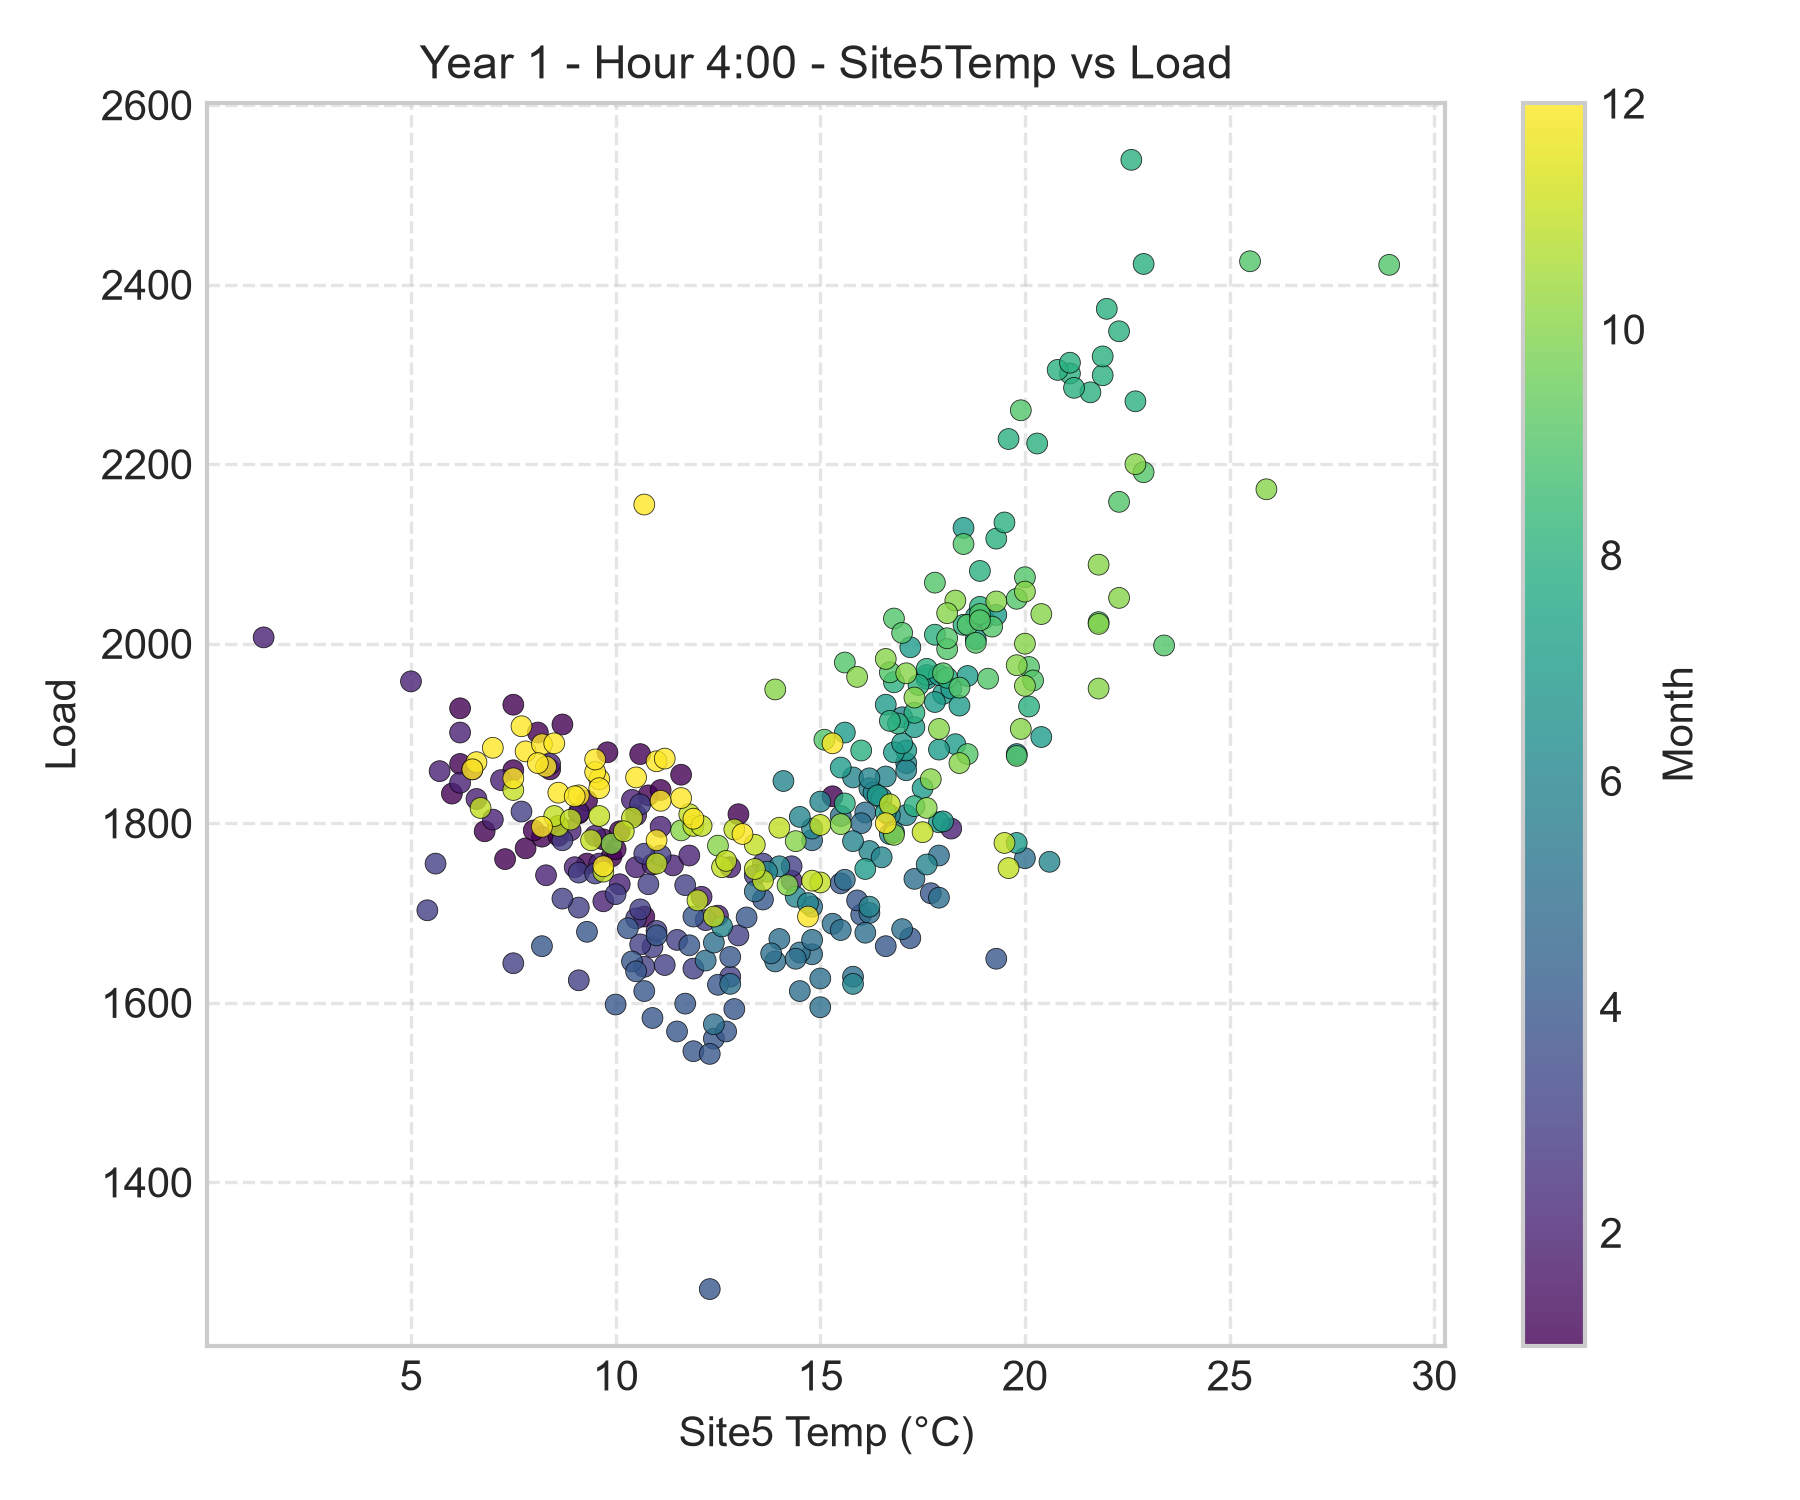
\includegraphics[width=\textwidth]{figures/Figure_1_Load_vs_Site5Temp_Year1.png}
        \caption{Năm thứ nhất (2020)}
    \end{subfigure}
    \hfill
    \begin{subfigure}[b]{0.48\textwidth}
        \centering
        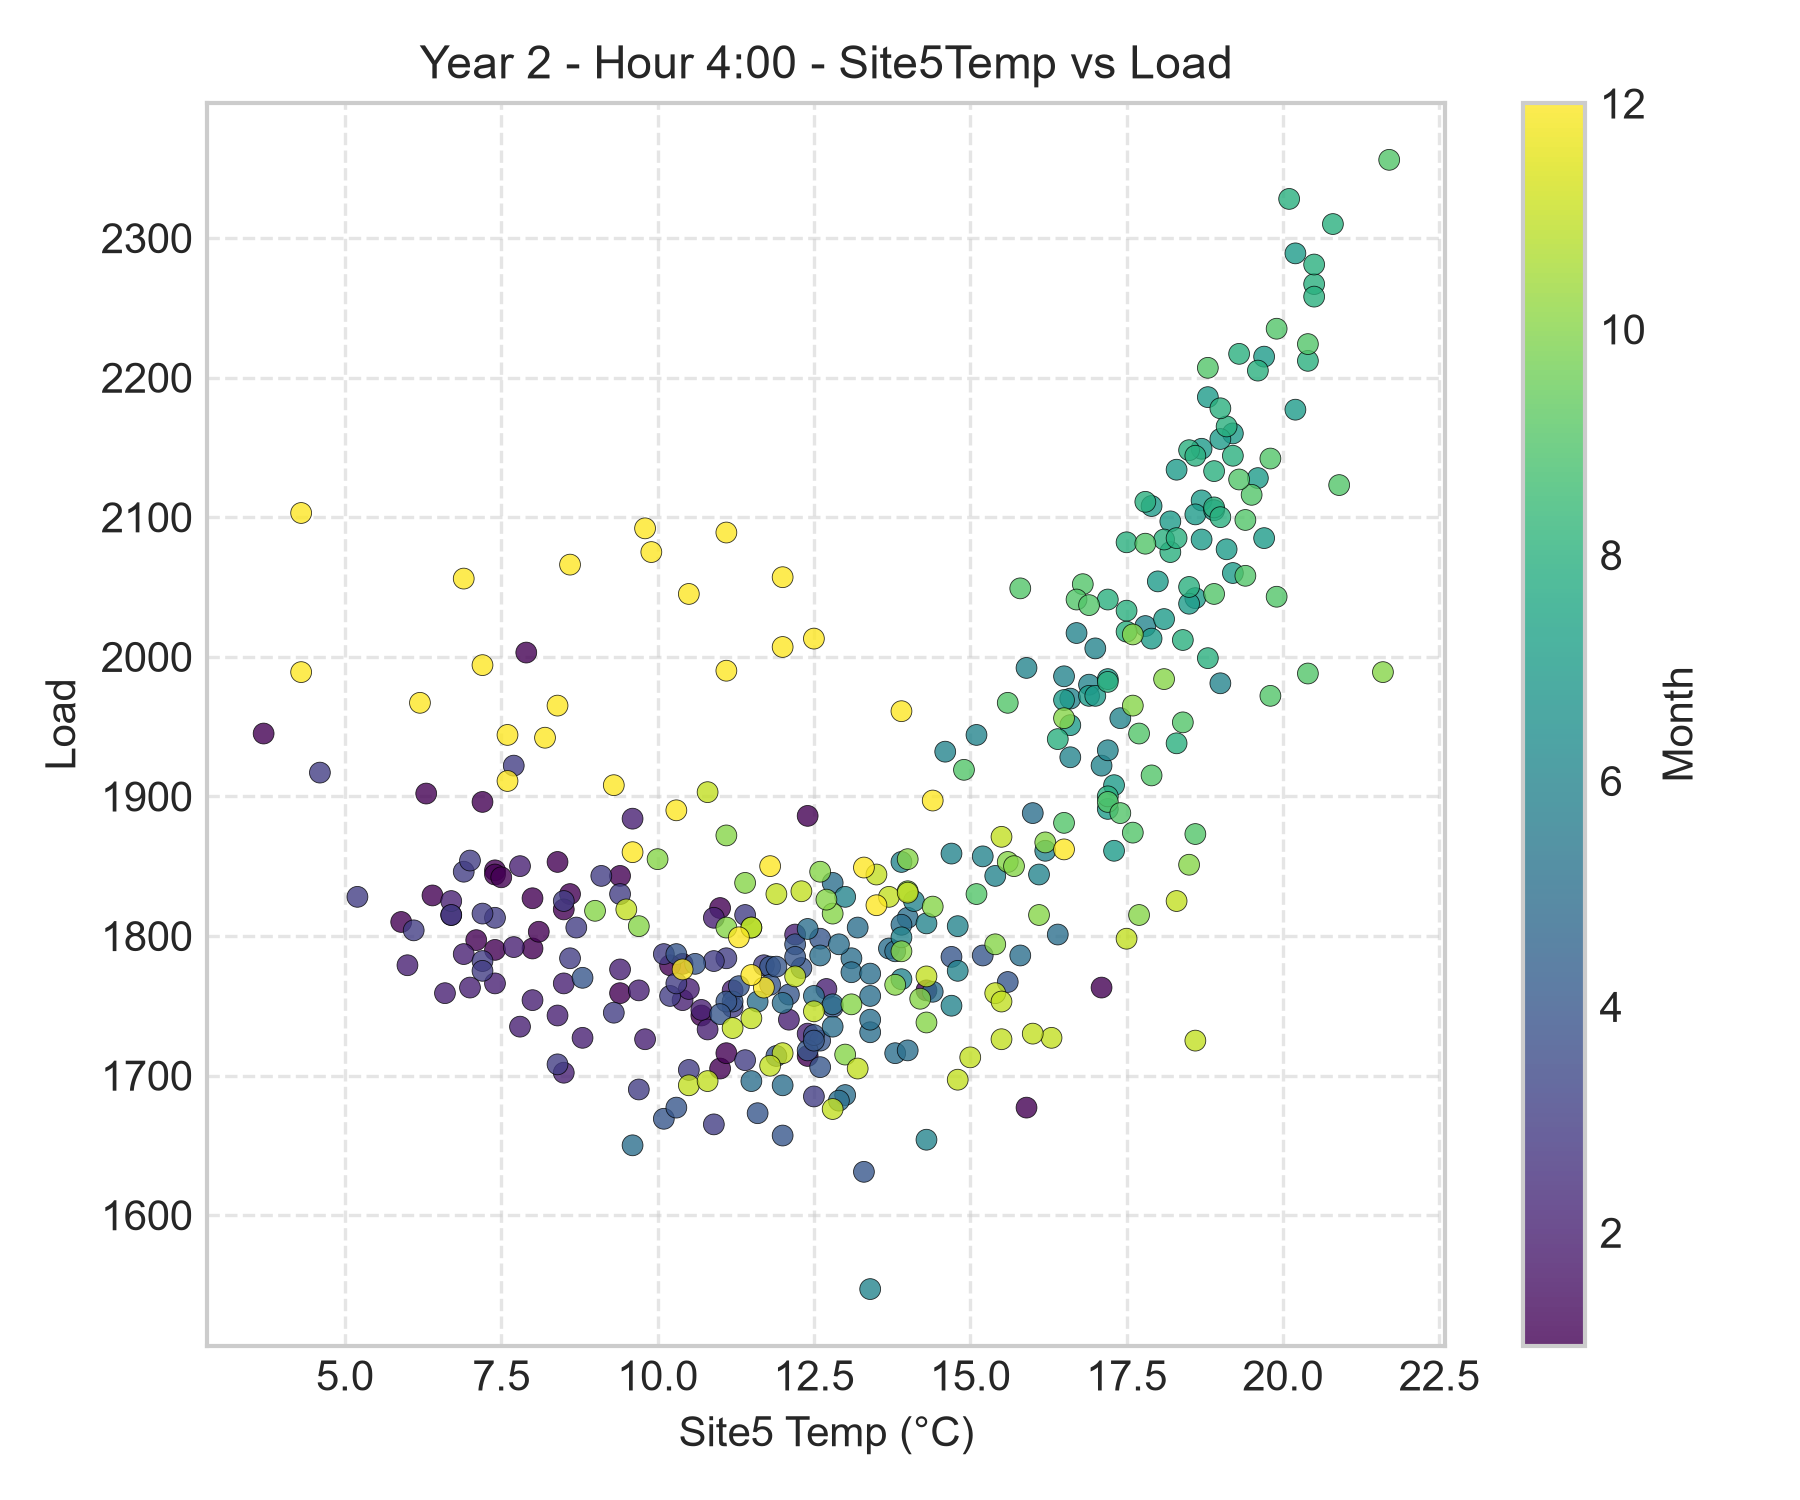
\includegraphics[width=\textwidth]{figures/Figure_2_Load_vs_Site5Temp_Year2.png}
        \caption{Năm thứ hai (2021)}
    \end{subfigure}
    \caption{Tương quan phi tuyến tính chữ U giữa phụ tải điện và nhiệt độ tại Trạm 5.}
    \label{fig:eda_temp_load}
\end{figure}

Hình~\ref{fig:eda_temp_load} thể hiện đồ thị phân tán giữa phụ tải điện và nhiệt độ tại Trạm 5 trong hai năm huấn luyện. Đường cong tương quan biểu hiện dạng chữ U sắc nét: phụ tải đạt mức tối thiểu tại khoảng nhiệt độ tiện nghi $17^\circ\text{C}$--$19^\circ\text{C}$, và tăng phi tuyến tính rất dốc khi nhiệt độ vượt quá $25^\circ\text{C}$, minh chứng xác thực cho sự cần thiết của các đặc trưng ngưỡng vật lý HDD và CDD. Ngoài ra, sự khác biệt về mẫu hình phụ tải giữa ngày làm việc và ngày cuối tuần được thể hiện rõ nét trong Hình~\ref{fig:eda_weekdays}, cho thấy phụ tải công nghiệp và thương mại giảm mạnh vào thứ Bảy và Chủ Nhật.

\begin{figure}[htbp]
    \centering
    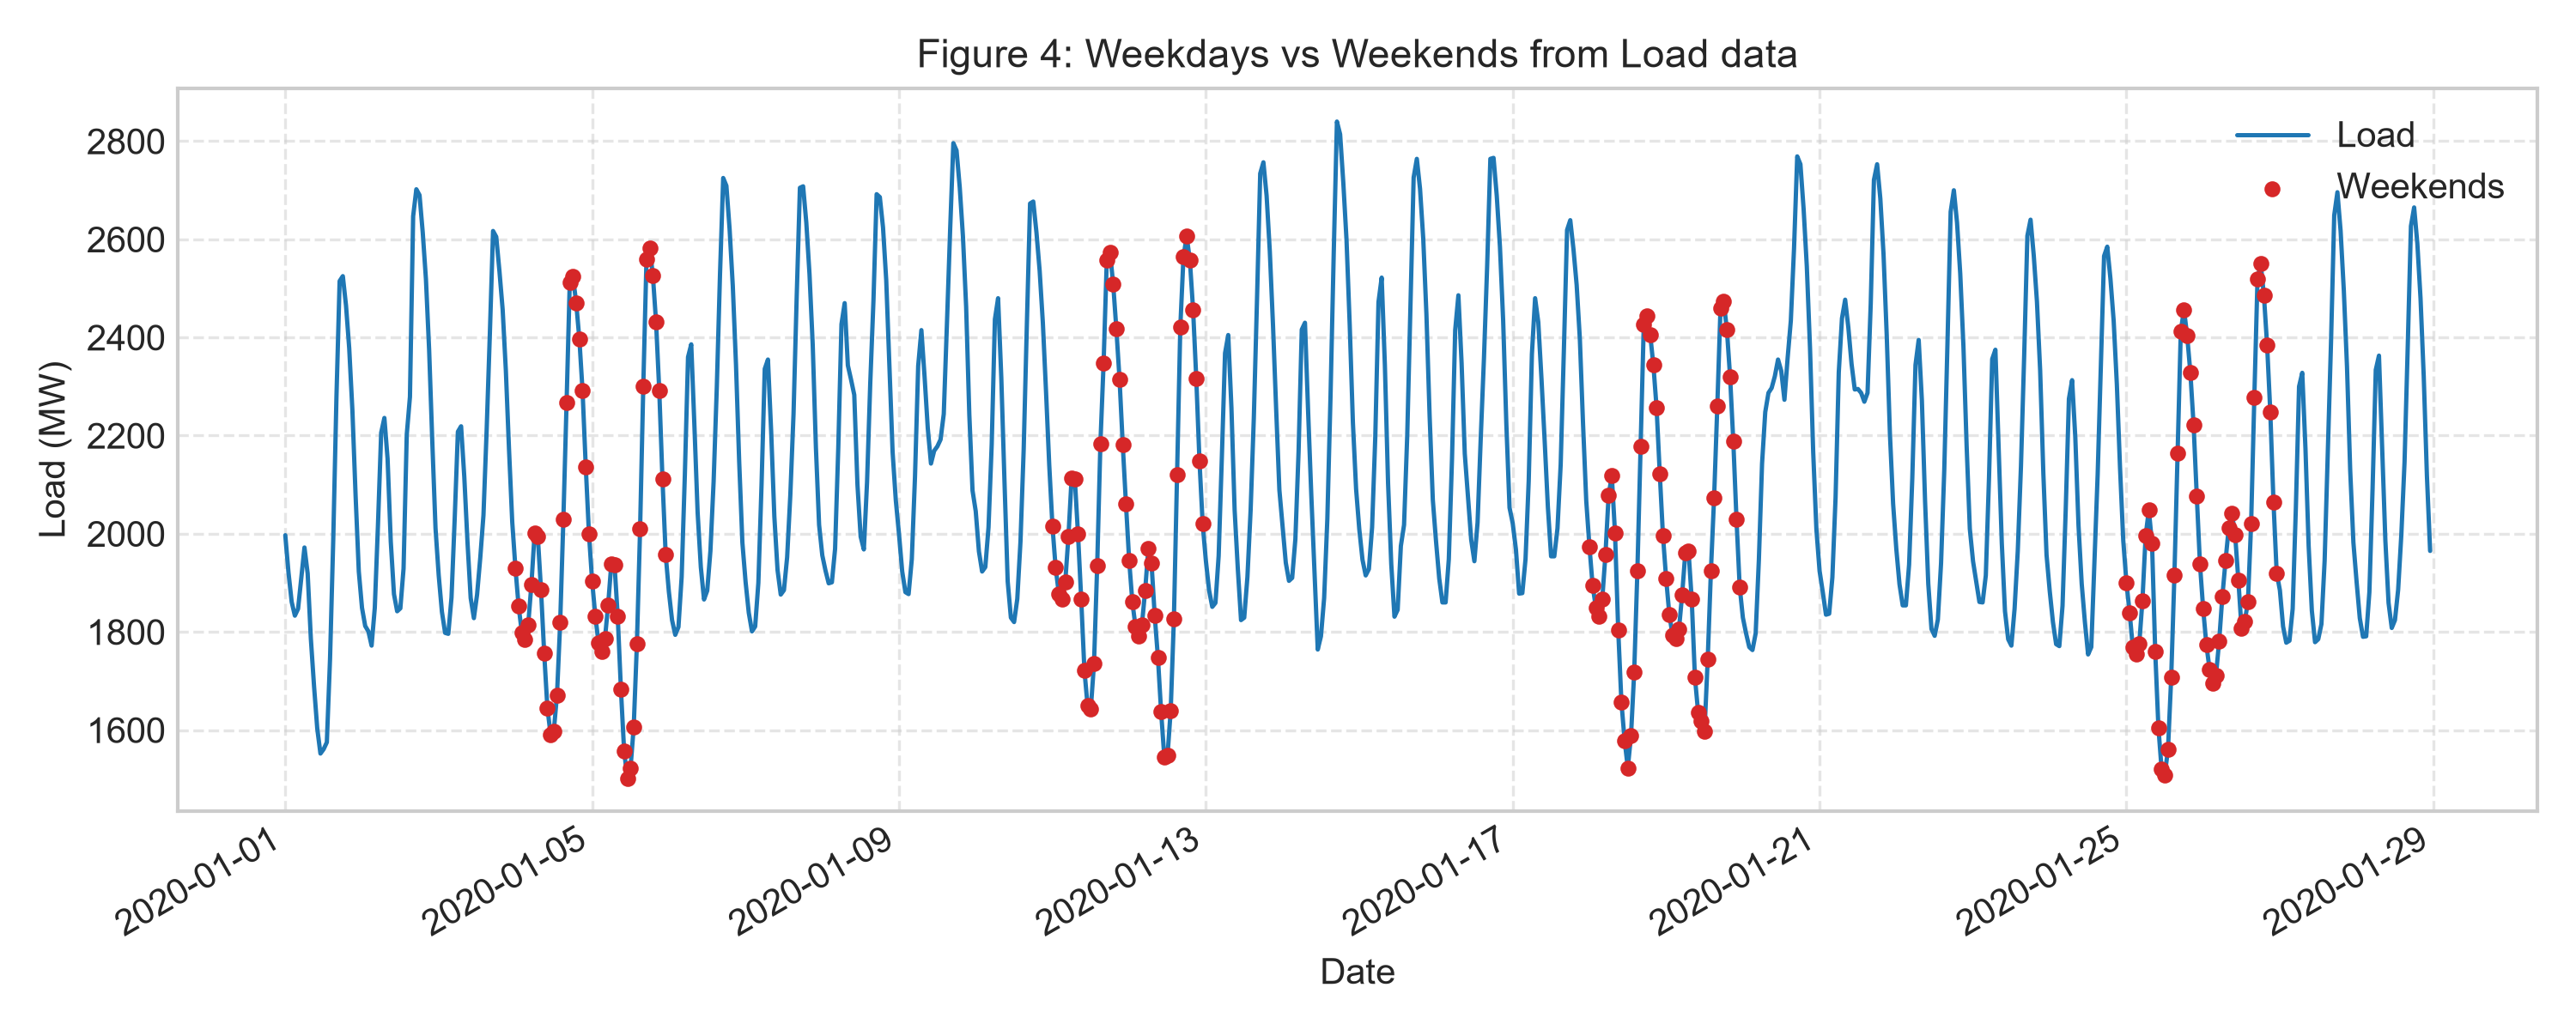
\includegraphics[width=0.75\textwidth]{figures/Figure_4_Weekdays_vs_Weekends.png}
    \caption{Phân phối đồ thị phụ tải giờ giữa Ngày làm việc và Ngày cuối tuần / Nghỉ lễ.}
    \label{fig:eda_weekdays}
\end{figure}

\subsection{Thiết kế So sánh và Các Giao thức Đánh giá}
Để đảm bảo tính khách quan và chống rò rỉ dữ liệu xuyên thời gian (\textit{temporal data leakage}), mọi phép biến đổi đặc trưng (fit ma trận chiếu PCA, tính giá trị trung bình hay độ lệch chuẩn) đều chỉ được thực hiện trên tập dữ liệu huấn luyện, sau đó áp dụng phép chiếu sang tập kiểm tra. Bốn giao thức kiểm thử chuẩn hóa được áp dụng:
\begin{enumerate}
    \item \textbf{Giao thức 1 (Year 1 $\to$ Year 2 Walk-Forward):} Huấn luyện trên Năm 1 (2020) và đánh giá trên Năm 2 (2021).
    \item \textbf{Giao thức 2 (Year 2 $\to$ Year 1 Generalization):} Huấn luyện trên Năm 2 (2021) và đánh giá trên Năm 1 (2020) để kiểm tra tính đối xứng.
    \item \textbf{Giao thức 3 (5-Fold Time-Series Cross-Validation):} Chia 2 năm huấn luyện (17,544 giờ) thành 5 nếp gấp tịnh tiến thời gian theo cửa sổ mở rộng (\textit{expanding window}).
    \item \textbf{Giao thức 4 (Year 3 Unseen Test Benchmark):} Thước đo đối chuẩn cao nhất: huấn luyện trên toàn bộ 2 năm đầu (2020 và 2021) và dự báo trên 8,760 giờ độc lập của Năm thứ 3 (2022).
\end{enumerate}

Metric chính đánh giá là RMSE (tiêu chuẩn chính thức của cuộc thi IISE PG\&E). Các metric phụ gồm MAE, MAPE, sMAPE và $R^2$. Toàn bộ thí nghiệm đều cố định $\text{random\_state} = 42$ nhằm đảm bảo $100\%$ tính tái lập thực nghiệm.

\subsection{Cấu hình Thí nghiệm và Môi trường Thực thi}
\begin{itemize}
    \item \textbf{24-Hourly XGBoost:} Gồm 24 mô hình \texttt{XGBRegressor} hoạt động song song. Cấu hình chuẩn: $200$ cây quyết định, $\text{max\_depth} = 6$, tốc độ học $\eta = 0.05$, $\text{subsample} = 0.8$, hàm mục tiêu hồi quy bình phương tối thiểu (\texttt{reg:squarederror}).
    \item \textbf{ElasticNet:} Cấu hình hệ số phạt $\alpha = 0.1$, $\text{l1\_ratio} = 0.5$ (chia đều chuẩn $L_1$ và $L_2$), $\text{max\_iter} = 2,000$.
    \item \textbf{Meta-Learner LightGBM:} Tinh chỉnh tự động qua 15 trials Optuna trên 3 nếp gấp TimeSeriesSplit OOF với không gian: $\text{n\_estimators} \in [50, 250]$, $\text{max\_depth} \in [2, 6]$, $\text{learning\_rate} \in [0.01, 0.2]$, $\text{num\_leaves} \in [7, 31]$, $\text{reg\_alpha} \in [10^{-3}, 5.0]$, $\text{reg\_lambda} \in [0.1, 10.0]$.
\end{itemize}
Thí nghiệm triển khai trên Python 3.10 với \texttt{xgboost 2.0.3}, \texttt{lightgbm 4.3.0}, \texttt{scikit-learn 1.4.1}, \texttt{optuna 3.5.0}, \texttt{shap 0.44.1}. Nhờ tính toán phân tán đa luồng (\texttt{n\_jobs=-1}), toàn bộ pipeline hoàn tất trong dưới 3 phút trên máy trạm thông thường.
